\graphicspath{{03_task_formulation/figures/}} % Location of the graphics files

\chapter{Task Formulation under Continuous and Partially-Observable Context}
\label{03_chp:task_formulation}

Common grounding is the process of creating, repairing and updating mutual understandings, which is a critical aspect of sophisticated human communication. However, existing dialogue systems still have limited capability of creating common ground, and we also lack task formulations which introduce natural difficulty of common grounding while enabling easy evaluation and analysis of complex models. In this chapter, we propose a minimal dialogue task which requires advanced skills of common grounding under \textit{continuous} and \textit{partially-observable} context. Based on this task formulation, we developed OneCommon Corpus: a large-scale dataset of 6,760 dialogues which fulfills essential requirements of natural language corpora. Through our dataset analysis, we uncover the difficulty of common grounding and other relevant phenomena that need to be considered. Finally, we evaluate and analyze baseline neural models on a simple subtask that requires accurate recognition of the created common ground. Our results show that the baseline models perform decently but leave room for further improvement.

\section{Introduction}
\label{03_sec:introduction}

One major goal of NLP is to develop systems with human-level competence of dialogue. In the field of psychology, the ability to construct and maintain common ground has been pointed out to be essential for natural language communication \citep{clark1996using} as well as acquisition \citep{tomasello2009constructing}. Furthermore, in human-computer interaction (HCI), it is important that humans and computers have certain ways of creating \emph{mutual understandings} to collaborate reliably \citep{brennan1998grounding}. Although natural language is not the only option, it is one of the most effective, effortless and versatile solutions to this problem.

\subsubsection{Problems of Existing Research}

However, existing study of common grounding in dialogue system research is limited in three major ways. First, existing dialogue tasks are limited in terms of common grounding due to the restricted types of information that need to be dealt with. Specifically, they are focused on either \emph{categorical} or \emph{fully-observable} context, which makes common grounding a relatively trivial task:

\begin{itemize}
  \item Under \emph{categorical} context \citep{bordes2017learning,he2017learning,lewis-etal-2017-deal}, information can be expressed by symbolic natural language with minimal ambiguity. For example, there could be little ambiguity in describing categorical attributes like discrete colors (``red'', ``blue'' and ``yellow''). However, under \emph{continuous} context, natural language usage becomes more nuanced and pragmatic (such as ``darker gray'' and ``almost black'') for precise semantic coordination.
  \item Under \emph{fully-observable} context \citep{zarriess-etal-2016-pentoref,de2017guesswhat}, it is usually given that every information about the context is shared among the agents. This makes common grounding easier because information of the context is already present in (or at least easily added to) their common ground. In contrast, under \emph{partially-observable} context, agents typically need to create common ground from minimal shared information, and there could be various misunderstandings or partial understandings that need to be resolved.
\end{itemize}

Another problem is the difficulty of evaluation and analysis. As the models acquire more flexibility, automatic evaluation becomes problematic \citep{liu2016,novikova2017} and interpretation of model behavior becomes more challenging. Since advanced common grounding requires high flexibility, it is expected that we will need reliable evaluation metrics and analysis methods in the process of comparing and improving different methods.

Finally, there are limitations of model capabilities. Although traditional dialogue systems rely on rule-based engineering and predetermined slot-filling \citep{traum1994computational,young2013pomdp,williams2016dialog}, these models lack flexibility in terms of representing dialogue states and generating natural utterances. Since common ground can be very complex involving high ambiguity, uncertainty, partial understandings and misunderstandings, we need systems that can better capture such complexities and resolve them through flexible dialogues.

\subsubsection{Our Contributions}

In this chapter, we make a first step towards addressing these problems in the following ways. First, we formulate a novel dialogue task which requires advanced skills of common grounding under \emph{continuous} and \emph{partially-observable} context. Our task is based on a more general \emph{collaborative reference task}, where the goal of the agents is to coordinate attention on the same entity in a given context. This setting enables clear evaluation based on the task success rate and various error analyses of arbitrary models, since the contexts are simple and completely controllable (Section \ref{03_sec:task_formulation}).

Second of all, to enable the development of recent end-to-end dialogue systems with high flexibility \citep{bordes2017learning,lewis-etal-2017-deal}, we collected a large-scale dataset of 6,760 human-human dialogues with over 32K utterances through crowdsourcing on Amazon Mechanical Turk. During the dataset collection, we defined and managed to fulfill three essential requirements of natural language corpora: namely interpretability, linguistic/strategic variety and reliability (Section \ref{03_sec:dataset_collection}).

Next, we conduct comparative analyses with the previous dataset to illustrate how continuous and partially-observable context introduces difficulty in terms of common grounding. In addition, we conduct further analyses of the dataset to investigate the common grounding strategies at different levels, including nonlinguistic bias towards \emph{joint saliency} (Section \ref{03_sec:dataset_analysis}).

Finally, we evaluate and analyze simple neural network models on our dataset based on an important subtask of collaborative reference. Due to the complexity of common grounding, there remains huge room for further improvement (Section \ref{03_sec:experiments}).

Overall, the contributions of this chapter are as follows:

\begin{itemize}
  \item We proposed a simple and general idea of incorporating continuous and partially-observable context to the dialogue tasks, which makes common grounding difficult in a natural way.
  \item Following this idea, we formulated a minimal collaborative reference task which enables clear evaluation and analysis of complex models.
  \item We collected a large-scale dataset of 6,760 dialogues, which fulfills essential requirements of natural language corpora.
  \item Our analysis of the dataset verified the difficulty of common grounding and revealed various phenomena that need to be considered.
  \item We evaluated simple baseline models on an important subtask of collaborative reference and demonstrated huge room left for improvement.
\end{itemize}

\section{Task Formulation}
\label{03_sec:task_formulation}


\begin{figure}[th!]
\center
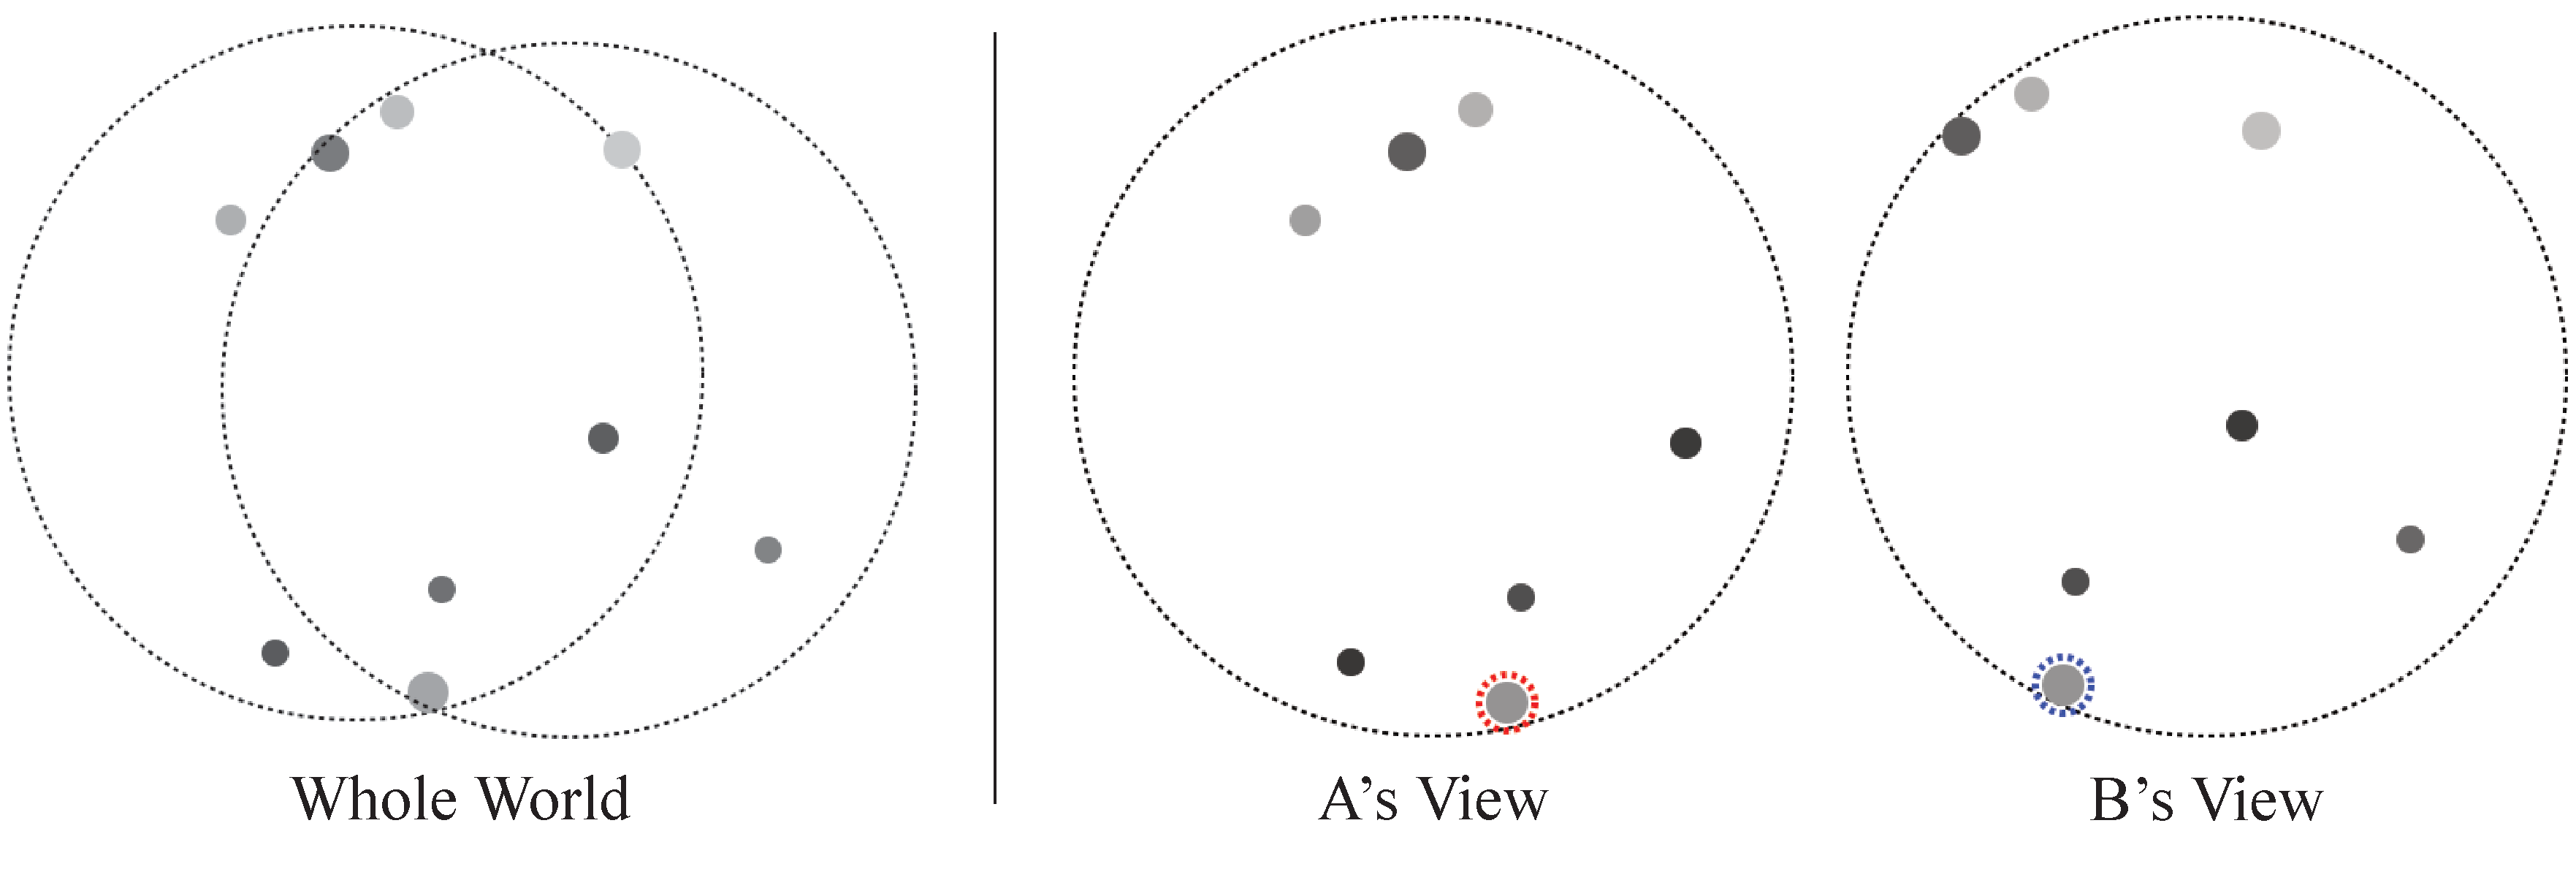
\includegraphics[width=\columnwidth]{onecommon_example.pdf}
\scalebox{0.95}{
\small
\begin{tabular}{@{}l@{}}
\toprule
A: I see three in a line going up and to the right. The middle one is the largest and darkest \\
B: I don't see that. I have one large, medium gray dot that's under a small, darker gray dot \\
A: Is the larger dot slightly to the left \\
B: yes, slightly, let's choose the larger one. \\
A: SELECT {\color{red} red} \\
B: SELECT {\color{blue} blue} \\
\bottomrule
\end{tabular}
}
\caption{An example dialogue of our collaborative reference task. Two agents have partial (overlapping) observations of a 2-D plane with 7 entities in each view. Their goal is to find and select the same entity through natural language communication.
}
\label{03_fig:onecommon_dialog}
\end{figure}

A \textit{collaborative reference task} is a multi-agent cooperative game with entities $E = \{e_1, e_2, ... , e_m\}$ and agents $A = \{a_1, a_2, ... , a_n\}$. Each agent $a_i \in A$ has an observation of $E$, and they can freely exchange information with other agents in natural language. At the end of the game, each agent selects one of the observable entities, and the game is considered \emph{successful} if and only if all the agents selected the same entity. This is a general framework for evaluating accurate \textit{mutual recognition} of a common entity, which is often a critical step in general common grounding.

Note that in contrast to the typical reference tasks \citep{kazemzadeh2014referit,de2017guesswhat}, agent roles are \textit{symmetric} and they can agree on any of the common entities (as long as it's the same). A dataset closest to our setup is the MutualFriends dataset \citep{he2017learning}, which is based on the task of finding a mutual friend from private lists of friends. Although this can be considered as a collaborative reference task under \emph{partially-observable} context (due to the privacy of knowledge), they only include \emph{categorical} information and the difficulty of common grounding is limited. 

Based on this task formulation, we propose a minimal task setting under \emph{continuous} and \emph{partially-observable} context. To be specific, we consider two agents and multiple entities located on a 2-D plane. Each entity has 3 simple attributes (2-D location, size and color) represented as \textit{continuous} real values. Furthermore, the agents are located slightly differently on the plane, and they can only observe the entities within a fixed radius: this way, our setting is made \textit{partially-observable} as well. 

We show an example dialogue of our task in Figure \ref{03_fig:onecommon_dialog}. Although human players successfully coordinated their selections with a short number of utterances, we can verify advanced common grounding strategies such as pragmatic expressions (\utterance{three in a line going up}), clarifications based on hypothesis testing (\utterance{Is the larger dot slightly to the left}) and nuanced acknowledgements (\utterance{yes, slightly}).

For the sake of simplicity, the number of entities observable by each agent is fixed at $7$. This ultimately reduces our task to a simple \textit{classification} problem, which can be evaluated based on simple metrics (such as accuracy).


\section{Dataset Collection}
\label{03_sec:dataset_collection}

We basically followed the dataset collection procedure of the MutualFriends dataset \citep{he2017learning}. We used Amazon Mechanical Turk to pair up 2 crowd workers and gave 20 seconds to read an example dialogue, followed by a maximum of 6 minutes session to complete the task. Our chat interface is shown in Figure \ref{03_fig:annotation}.

\begin{figure}[ht]
\centering
\vspace{1mm}
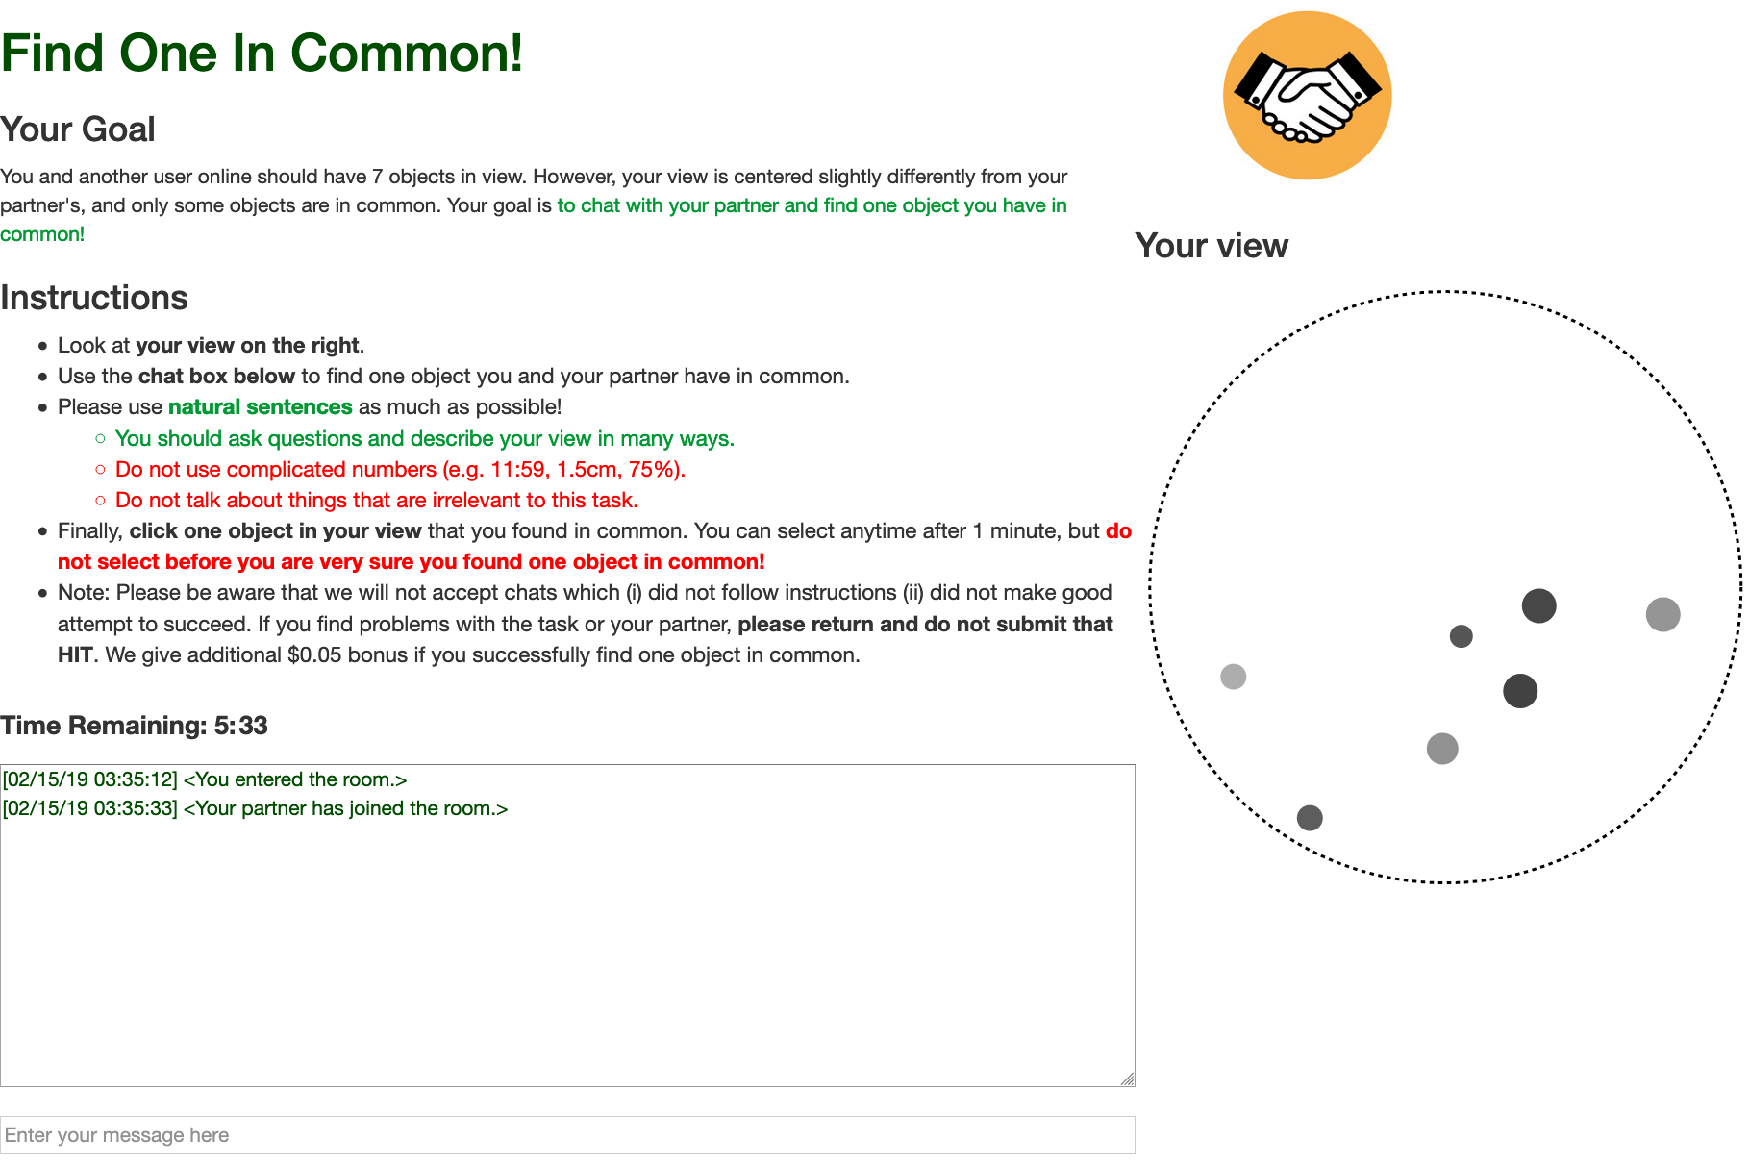
\includegraphics[width=0.95\columnwidth]{annotation.pdf}
%\vspace{1mm}
\caption{
A screenshot of our chat interface. Workers are given a maximum of 6 minutes to identify one of the common entities through dialogue.
}
\label{03_fig:annotation}
\end{figure}

In this procedure, we were concerned with three essential requirements of natural language corpora: namely \emph{interpretability}, \emph{linguistic/strategic variety} and \emph{reliability}. In the following, we discuss the importance of each requirement as well as how we managed to fulfill them:
\\

\noindent
\textbf{Interpretability}\quad
We define the interpretability of the dataset to be the ease of interpreting its language and strategy, which is critical for conducting annotations and further analyses. However, \emph{lack of discipline} and \emph{complexity of the vocabulary} can make corpora difficult for interpretation.

In free-formed dialogues, lack of discipline can cause unnecessary difficulty in terms of interpretation. For instance, \emph{cross-talk} (conversation which does not progress sequentially) can occur frequently \citep{he2017learning} and complicate important structures of dialogues, such as discourse segments, adjacency pairs and \emph{contributions} in common grounding \citep{clark1989contributing}. Hence, we minimized them by forcing workers to take turns. Also, \emph{chit-chat} could occur occasionally, which adds undesirable noise for analyzing common grounding. Therefore, we explicitly instructed the workers to avoid talking about things that are irrelevant to this task.

Keeping the vocabulary simple is also important for interpretability, especially for people unfamiliar with the domain. For instance, the MutualFriends dataset includes up to 7 attributes with approximately 3K complex named entities and technical terms. In contrast, we kept the entity attributes minimal with only 3 simple and intuitive properties (location, size and color). As a result, this greatly reduced the complexity of the vocabulary as we describe in Section \ref{03_sec:dataset_analysis}.
\\

\noindent
\textbf{Linguistic and Strategic Variety}\quad
\emph{Linguistic and strategic variety} of the dataset is fundamental for developing dialogue systems with broad coverage. To satisfy this requirement, we sampled all entity attributes randomly from fixed uniform distributions, with the only restriction that the entities cannot be too close to each other. As the previous work with the similar idea confirmed \citep{suhr2017corpus}, we found rich varieties of linguistic phenomena, including cardinalities (\utterance{\textit{three} gray dots}), existentials (\utterance{\textit{There is} another small dark ..}), universals (\utterance{\textit{all} of the other dots are larger}), coordinations and negations (\utterance{further to the right \textit{and} \textit{not} as far down}).

During the dataset collection, we assigned 6,759 unique contexts to 6,760 dialogues we collected. We collected 2 dialogues based on the exact same context and confirmed that they solved the task in different ways. This suggests that there could be various effective solutions and the agents must adapt flexibly to their partners' strategies.

Finally, we incorporated variation in terms of the \textit{degree} of partial observability. Specifically, each agent has 7 entities in the view, but only 4, 5 or 6 of them would be in common. This introduces a further variation of common grounding strategies, as we discuss in detail in Section \ref{03_sec:dataset_analysis}.
\\

\noindent
\textbf{Reliability}\quad
Finally, we regard the \emph{reliability} of the dataset to be crucial, especially when crowdsourcing data with potentially careless, low-motivated workers. In fact, in our preliminary experiment, we found many cases where workers did not follow the instruction carefully or solve the task effectively (especially on difficult cases).

As a solution, we manually reviewed all works and rejected ones which clearly did not follow the instruction. Our instruction is kept brief and explicit so that it is easier to follow, and we also gave manual feedback about general solutions to improve their work. To discourage premature guessing, we prohibited workers from selecting within the first minute and instructed them to make it \emph{very sure} they found the same entity before selection. We also incentivized task success with \$0.05 bonus for all successful dialogues, in addition to the base reward of \$0.30.

As a result, we found significant improvement in terms of task success rate, which is an important evidence of the reliability of our dataset. \\

Based on the above procedure, we collected 6,839 dialogues, and after the reviewing process, we accepted 6,760 dialogues in total. We refer to this dataset as \textbf{OneCommon Corpus}. Overall, we received positive feedback from the crowd workers and they seemed to enjoy playing it, which is important from the aspect of gamification.

\section{Dataset Analysis}
\label{03_sec:dataset_analysis}

In this section, we first study the difficulty of common grounding in comparison to the previous settings. Secondly, we conduct further analyses to investigate other relevant phenomena that need to be considered.

\subsection{Difficulty of Common Grounding}
\label{03_subsec:difficulty_analysis}

Our hypothesis is that \emph{continuous} and \emph{partially-observable} context makes common grounding difficult compared to \emph{categorical} or \emph{fully-observable} context. However, it is relatively obvious that \emph{fully-observable} setting would make collaborative reference trivial: for instance, if our task was fully-observable, one can easily succeed by always uttering \utterance{\textit{select the leftmost dot}}. Therefore, we mainly focus on assessing how \textit{continuous} context adds difficulty in terms of common grounding.

As a comparison, we use the MutualFriends dataset which is based on a similar collaborative reference task under partially-observable but \emph{categorical} context \citep{he2017learning}. However, several differences make a direct comparison difficult: for instance, we only gave one chance for the entity selection, while the MutualFriends dataset allowed multiple chances in the given amount of time. Therefore, we focus on the following factors which are less affected by such differences.

\subsubsection{Utterance Lengths}

\begin{table*}[ht]
\centering \scalebox{0.81}{
%\setlength\tabcolsep{9pt}
\setlength{\aboverulesep}{0pt}
\setlength{\belowrulesep}{0pt}
\setlength{\extrarowheight}{.2ex}
\begin{tabular}{c|cccc}
\toprule
 & \multirow{2}{*}{MutualFriends} & \multicolumn{3}{c}{OneCommon} \\
 & & \#Shared=4 & \#Shared=5 & \#Shared=6 \\
\midrule
Total dialogues &
10,661 & 2,189 & 2,279 & 2,292 \\
Average tokens per utterance&
5.38 & 12.87 & 12.37 & 11.86\\
Average utterances per dialogue&
8.97$^*$ & 4.97 & 4.77 & 4.56 \\
Success rate (\%) &
0.85$^*$ & 0.66 & 0.77 & 0.87 \\
\midrule
Unique tokens & 13,478 & \multicolumn{3}{c}{3,761} \\
Occupancy of top 10\% frequent tokens (\%) & 91.6\% & \multicolumn{3}{c}{97.0\%} \\
\bottomrule
\end{tabular}
}
\caption{\label{03_tab:statistics}
Basic statistics of our dataset and the MutualFriends dataset \citep{he2017learning}. To count tokens and vocabulary size, we preprocessed the text with the same NLTK word tokenizer \citep{nltkbook} and converted each token to its lowercased form. ($^*$ denotes where direct comparison is not suitable due to the task difference.)
}
\end{table*}

First, we compare the \emph{average utterance length} because this indicates the syntactic/semantic complexity of utterances required for common grounding. As shown in Table \ref{03_tab:statistics}, utterances in our dataset are at least twice as long compared to the MutualFriends dataset: this indicates that more complex utterances are required under continuous context to make the descriptions precise. We also found that the utterance lengths slightly increase when the number of shared entities is smaller: this suggests that (a greater degree of) partial-observability also adds complexity at the utterance level.

\subsubsection{Pragmatic Expressions}

\begin{figure}[th!]
\centering
\begin{tikzpicture}
\node[inner sep=0pt] (agent_0) at (0,0)
  {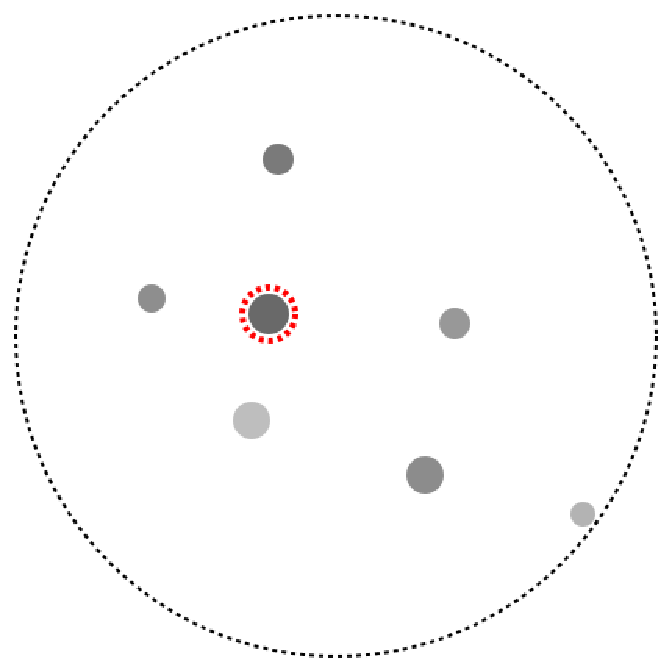
\includegraphics[width=0.35\columnwidth]{S_VdQsGMpy6Su1tzIy_agent_0.pdf}};
\node[inner sep=0pt] (agent_1) at (6,0)
  {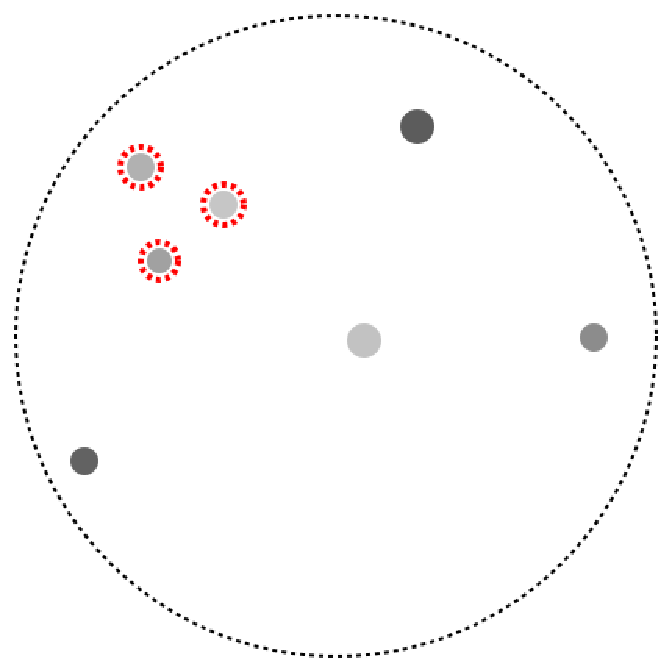
\includegraphics[width=0.35\columnwidth]{S_xJimjRbmhtdjZbNl_agent_1.pdf}};
\node [below] at (0,-2.5) {large \textbf{black} dot};
\node [below] at (6,-2.5) {a close \textbf{triangle}};
\end{tikzpicture}
\caption{
Examples of typical pragmatic expressions in our dataset (marked by bold).
}
\label{03_fig:pragmatics}
\end{figure}

In our dataset, we found many \emph{pragmatic expressions} whose meaning depends on the context and should not be taken literally. A typical example is the usage of the word ``black'' to indicate the darkest dot in the context, even if its color is not completely black. Another common expression ``triangle'' is also pragmatic, since in the literal sense there could be numerous triangles in one's view, and the speaker actually indicates a group of three dots which is the closest to a \textit{prototypical} type of triangles, such as an equilateral triangle. We show some illustrating examples in Figure \ref{03_fig:pragmatics}.

As the previous work pointed out, such pragmatic expressions are characteristic under continuous context \citep{monroe2017colors} and add complex ambiguity/uncertainty that need to be resolved through common grounding.

\subsubsection{Nuanced Expressions}

Finally, the frequent usage of \emph{nuanced} expressions is an important characteristic of our dataset. Since the context is continuous and partially-observable, we hypothesize that speakers need to rely on such expressions to express subtle differences in terms of degree, ambiguity, uncertainty, and so forth.

To estimate the frequency of nuanced expressions, we follow \citet{paradis_2008} and define 2 main types (and 5 subtypes) of degree modifiers: \textit{scalar modifiers} used for concepts in a range of scale (\textit{diminishers}, \textit{moderators}, \textit{boosters}) and \textit{totality modifiers} used for concepts with definite boundaries (\textit{approximators}, \textit{maximizers}). See Figure \ref{03_fig:degree_modifiers} for the proposed taxonomy and examples of such degree modifiers.

\begin{figure}[th!]
\center
\vspace{2mm}
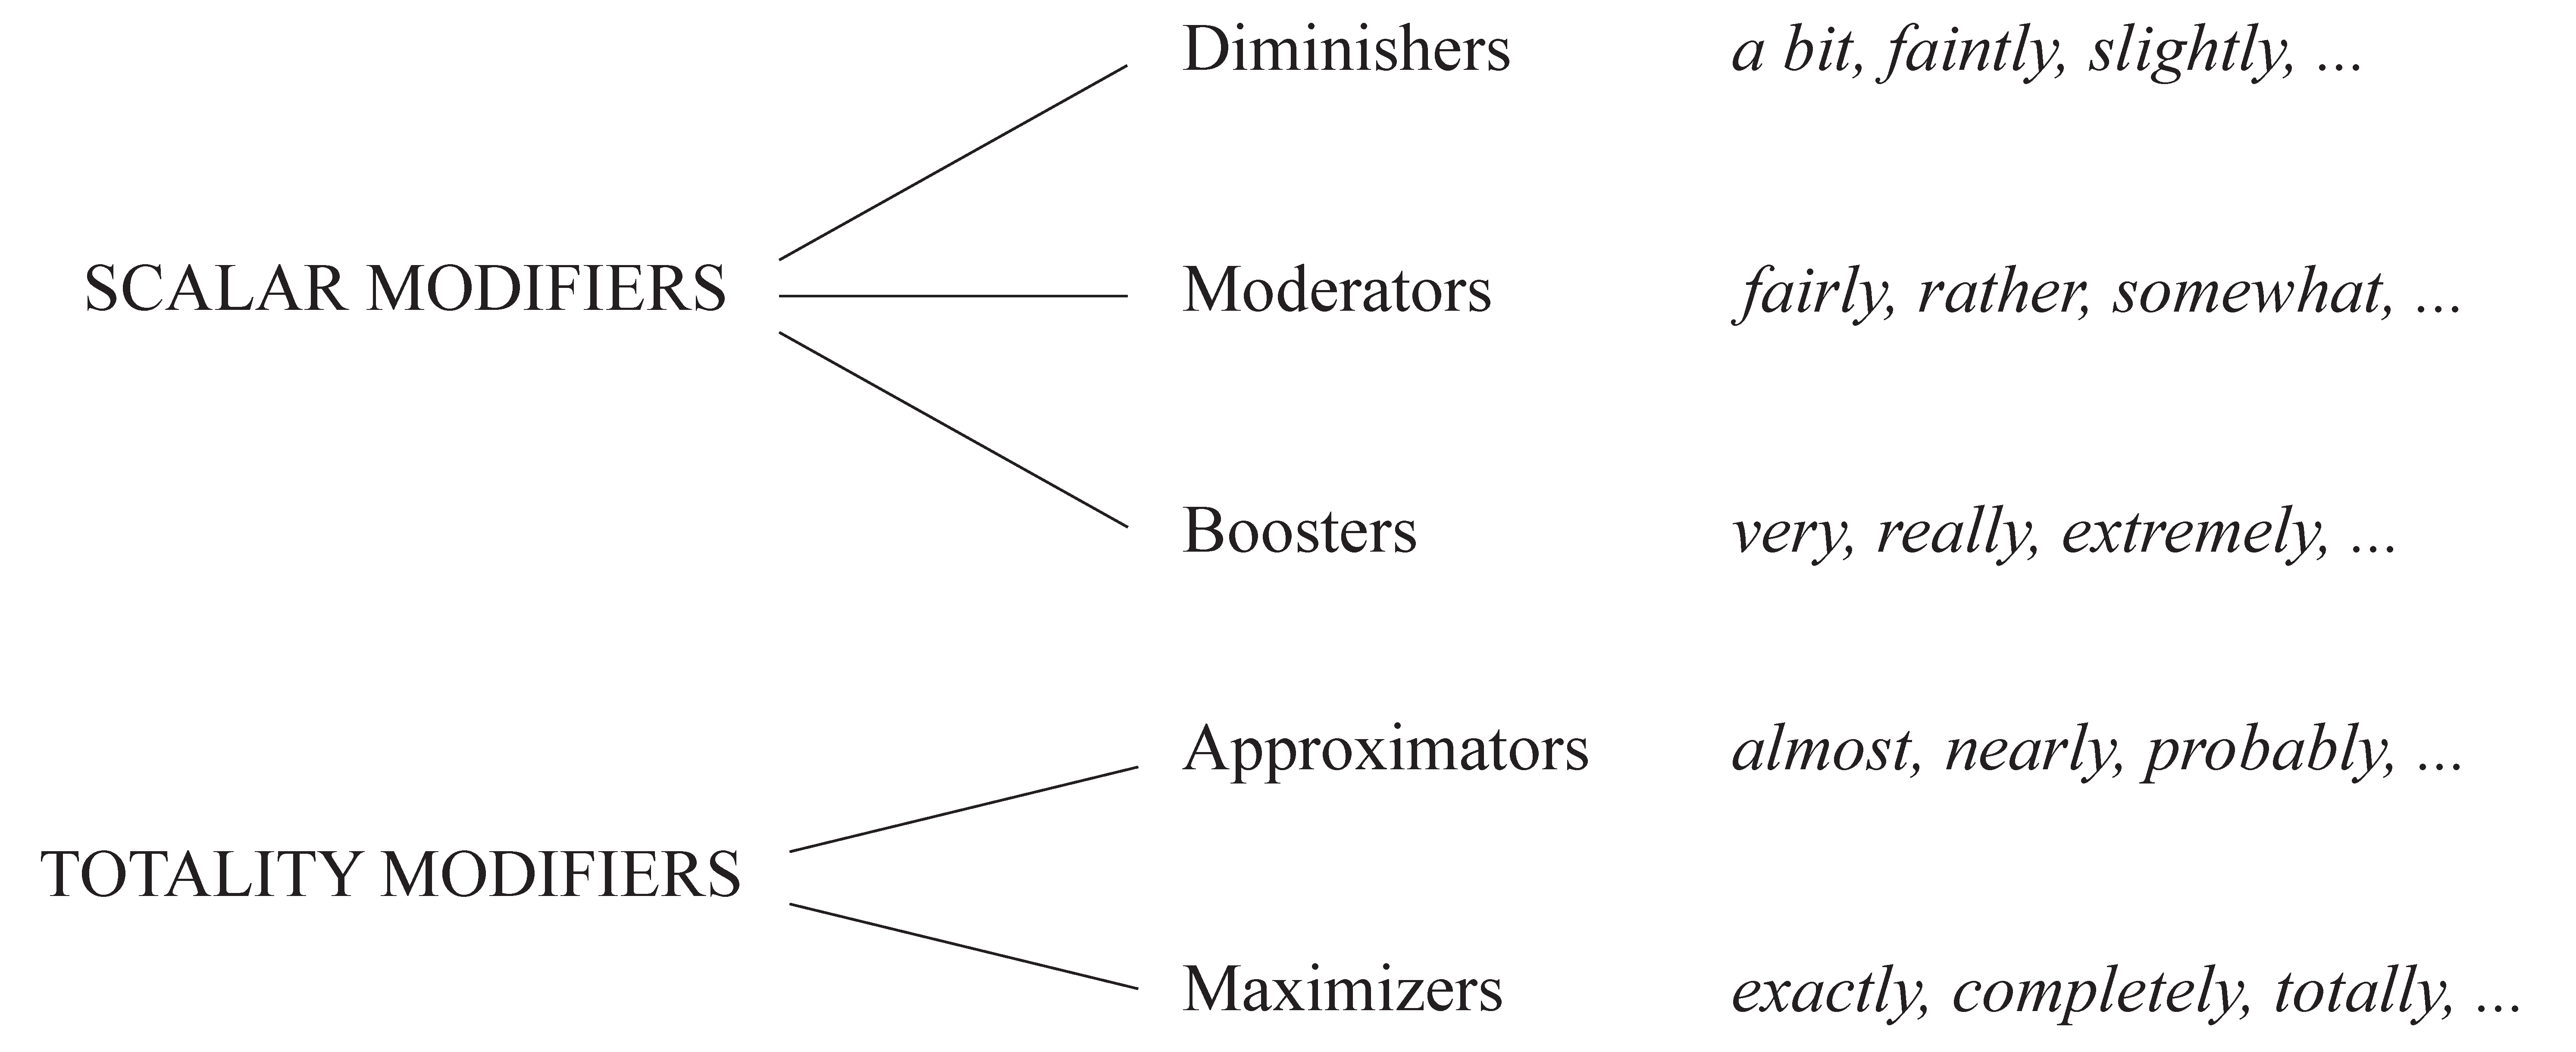
\includegraphics[width=0.97\columnwidth]{degree_modifiers.pdf}
\vspace{1mm}
\caption{A taxonomoy of the degree modifiers based on \citet{paradis_2008}.
}
\label{03_fig:degree_modifiers}
\end{figure}

Based on this taxonomy, we manually created a keyword-based dictionary of the degree modifiers. Note that we excluded words which are likely to be used with different meanings (such as ``like'', ``about'' and ``around'') and do not consider nuances expressed morphologically (such as \textit{-ish} as in ``small\textit{ish}''), although they are also common in our dataset. Using this dictionary, we estimated the frequency of the modifiers in the MutualFriends dataset and OneCommon Corpus. As shown in Table \ref{03_tab:nuances}, we can verify that our dataset includes significantly more degree modifiers of various types, which are used effectively to cope with ambiguity and uncertaintiy. \\

\begin{table*}[t!]
\centering \scalebox{0.83}{
\setlength\tabcolsep{9pt}
\setlength{\aboverulesep}{0pt}
\setlength{\belowrulesep}{0pt}
\setlength{\extrarowheight}{.4ex}
\begin{tabular}{c|cc|cl}
\toprule
Degree Modifiers & MutualFriends & OneCommon & \# Keywords &  \multicolumn{1}{c}{Usage in OneCommon} \\
\midrule
Diminishers & 0.01 & 9.19 & 10 & \textbf{slightly} to the right \\
Moderators & 0.09 & 1.28 & 6 & \textbf{fairly} close together \\
Boosters & 0.17 & 9.83 & 27 & \textbf{very} light dot \\
Approximators & 0.86 & 10.23 & 34 & \textbf{almost} in the middle \\
Maximizers & 0.47 & 4.31 & 37 & \textbf{exactly} horizontal \\
\bottomrule
\end{tabular}
}
\caption{\label{03_tab:nuances}
Average occurrences of degree modifiers per 100 utterances (estimated based on keywords).
}
\end{table*}

To summarize our analyses, utterances are much longer in our dataset, which indicates the complexity of common grounding at the utterance level. In addition, our dataset involves more ambiguity and uncertainty represented by the frequent usage of pragmatic and nuanced expressions. These observations verify that common grounding becomes more difficult and complicated under continuous and partially-observable context.

On the other hand, we found that human workers could solve the task reasonably well with little evidence of confusion. Therefore, we conclude that our task setting is fundamental for adding natural difficulty in terms of common grounding.

\subsection{Other Relevant Phenomena}

Next, we conduct further analyses of the dataset and investigate various phenomena related to common grounding that need to be considered.

\subsubsection{Basic Statistics}

From Table \ref{03_tab:statistics}, we also found that dialogues get longer in terms of the \emph{(average) number of utterances} when a fewer number of entities is shared. This shows that under a greater degree of partial-observability, it is more likely that the presented information is not \emph{groundable}, and players need more interaction (try-and-error) to create common ground. We can also see that the success rate drops naturally, so in general common grounding becomes more challenging when less information is shared.

In terms of lexical variety, our dataset contains 3,761 unique tokens in total, in contrast to 13,478 in the MutualFriends dataset. In addition, we found that a large portion of our dataset consists of common words: to be specific, the top 10\% of the most frequent tokens occupy 97.0\% of the whole tokenized corpus, in contrast to 91.6\% in the MutualFriends dataset. These suggest that the vocabulary of our dataset is extremely simple, which is an important evidence of interpretability discussed in Section \ref{03_sec:dataset_collection}. This may also be helpful for training dialogue systems, since rare words are less problematic.

\subsubsection{Nonlinguistic Phenomena}

Language is a \emph{coordination device} we use to coordinate our joint actions \citep{lewis1969convention}, but we also use \emph{joint saliency} to coordinate actions at the nonlinguistic level \citep{Schelling1960}. In our dataset, we found that human players have a tendency to focus attention on \emph{perceptually} salient entities more often.

To demonstrate this, we plot the final selection probabilities of the entity's color and size in Figure \ref{03_fig:plot-select}. We can clearly see that the selections are biased, and entities with extreme properties (around the edge) are more likely to be selected. We also found that darker entities are more likely to be selected (62.7\%) compared to lighter entities (37.3\%), and larger entities (54.3\%) slightly more likely than smaller entities (45.7\%).

There could be other types of joint saliency as well (such as geometric relations between entities), but the point is that such bias exists and needs consideration: for example, just by taking advantage of such bias, we can predict human selections significantly better than random (Section \ref{03_sec:experiments}). However, due to the \textit{partially-observability}, joint saliency is not sufficient and communication is critical to solving our task.

\begin{figure}[t!]
\centering
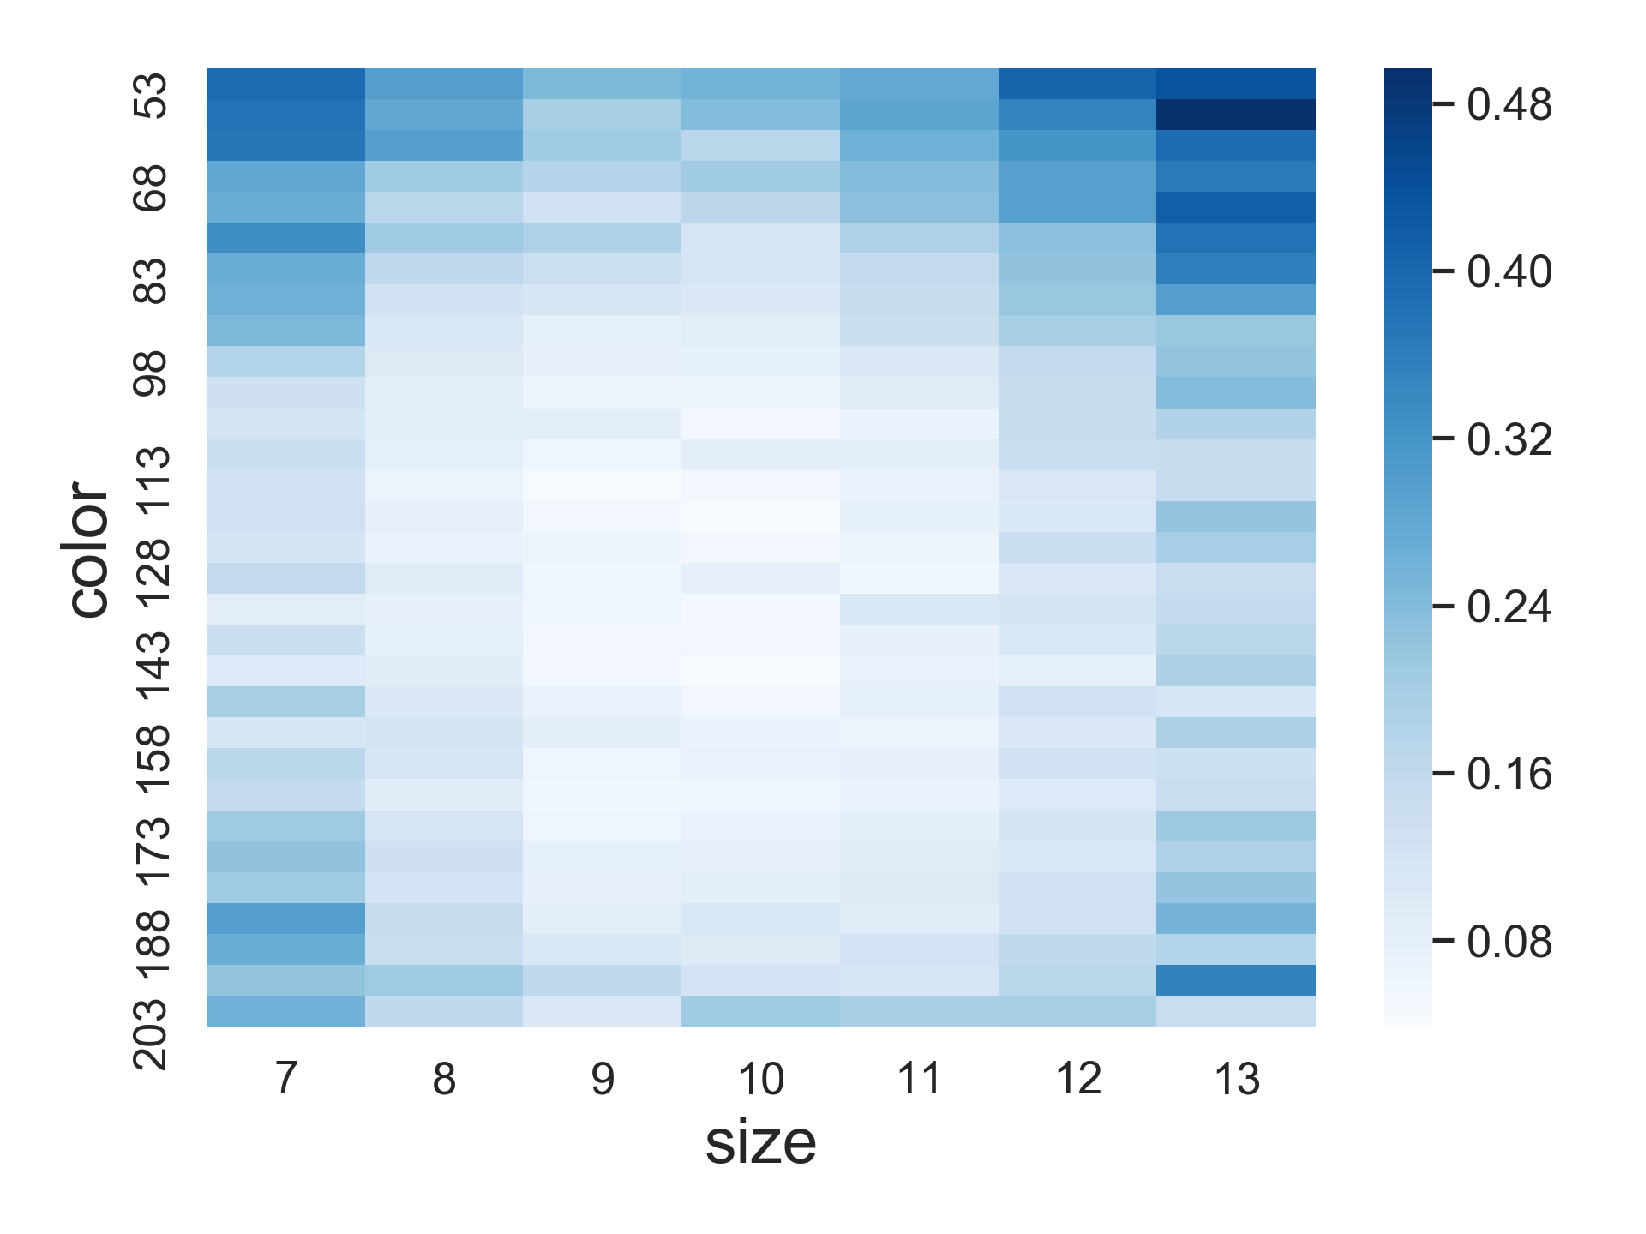
\includegraphics[width=0.74\columnwidth]{selection_bias.pdf}
\caption{
Final selection probabilities based on color and size. The total range of size is 7 and color is split into 30 equal-sized bins in grayscale (smaller is darker).
}
\label{03_fig:plot-select}
\end{figure}

\subsubsection{Utterance Level Phenomena}

Understanding speaker's intention at the \emph{utterance level} is critical in dialogue \citep{grice1957meaning}: especially the idea of speech act \citep{austin1962things,searle1969speech} has been applied widely in dialogue system research to improve natural language understanding and generation \citep{yao2013recurrent,hakkani2016multi}.

During data collection, we allowed free-formed conversation with minimal restrictions, as long as they are relevant to the accomplishment of the task. As a result, we found a wide variety of speech acts in the course of common grounding. We show illustrative examples of the collected utterances in Table \ref{03_tab:speechact}. Utterances are grouped by the \textit{communicative functions} defined in \citet{bunt2017dialogue}, including \textit{information transfer functions} (\textit{information provision/request}) and \textit{action discussion functions} (\textit{commissives/directives}). With additional annotations, our dataset can be easily extended to study such pragmatic structures as well \citep{stolcke-etal-2000-dialogue}.

\begin{table*}[th!]
\centering \scalebox{0.82}{
\begin{tabular}{lcl}
\toprule
Function & Type & Example Utterances\\
\midrule
\multirow{8}{*}{Info. Provision} & \multirow{1}{*}{Inform (Init.)} & I have very dark small dot in the center \\
& \multirow{1}{*}{Inform (Cont.)} & It also has a small light grey one further down from the group \\
& \multirow{1}{*}{Agreement} & Yes I have one like that. / same here. \\
& \multirow{1}{*}{Agreement (Strong)} & Exactly! / perfect. mine too. \\
& \multirow{2}{*}{Agreement (Partial)} & not sure its the one / more of a line. \\
& & Yes, but the small is medium dark, not completely black \\
& \multirow{1}{*}{Disagreement} & I don't have that one. / mine are not in those locations. \\
\midrule
\multirow{4}{*}{Info. Request} & \multirow{1}{*}{Question (Prop.)} & the middle one is the darkest of the 3? \\
& \multirow{1}{*}{Question (Set)} & where is it in relation to the large med grey? \\
& \multirow{1}{*}{Question (Choice)} & Which should we choose? / the black or the grey? \\
& \multirow{1}{*}{Question (Check)} & It's the darkest dot in the circle, right? \\
\midrule
\multirow{1}{*}{Commissives} & \multirow{1}{*}{Offer} & lets click the upper left one that's bigger and darker gray \\
\midrule
\multirow{2}{*}{Directives} & \multirow{1}{*}{Request} & tell me about your tiniest dot? / pick one at the bottom \\
& \multirow{1}{*}{Suggestion} & Please describe it in relation to other dots in the circle \\
\bottomrule
\end{tabular}
}
\caption{\label{03_tab:speechact}
Illustrative utterances in the dataset, grouped by the \emph{task dimension} of communicative functions \citep{bunt2017dialogue}}
\end{table*}

\subsubsection{Discourse Level Phenomena}

Finally, we found many coreferences and anaphoric expressions in our dataset. \emph{Coreference resolution} is the task of finding the mentions (referring expressions) in the dialogue with the same referents \citep{ng-2010-supervised}. In our dataset, we found two characteristics that complicate this task. First, due to the continuous and partially-observable context, mentions are usually ambiguous and the referents could be missing from one's view. Hence, players must keep track of various possibilities and disambiguate them through interaction. Secondly, players often use the \emph{grouping} strategy (such as ``three in a line'', ``a cluster of 4 dots'') where the mention can refer to a \emph{set} of multiple entities. This is a natural and effective strategy but adds complexity in terms of coreference resolution.

On the other hand, \emph{anaphora resolution} is the task of idenfitying the relation between a mention (\textit{antecedent}) and a succeeding mention (\textit{postcedent}) that depends on the previous mention \citep{poesio2016anaphora}. This can occur both within utterances (\utterance{a medium size black one, with a very light slightly smaller one to \textit{its} left}) and across utterances (\utterance{Does \textit{the lighter dot} appear to be slightly larger?}). In \textit{associative anaphora}, the referents of the postcedent can be different from the antecedent, e.g. only refer to a \textit{part of} the antecedent (as in \utterance{I have a pair where \textit{the left one} is large and dark}).

These discourse-level phenomena play a fundamental role in the process of common grounding and will be the main focus of our study in Chapter \ref{04_chp:interpretation}.

\section{Experiments}
\label{03_sec:experiments}

\subsection{Evaluation}

In this experiment, we focus on a simple subtask of common grounding, which we refer to as the \textbf{target selection task}. Specifically, our goal is to predict which target entity a human player selected, provided the player's private observation and the corresponding dialogue. This is an essential subtask of collaborative reference, where the player makes the final selection based on the established common ground. 

Since the number of entities in each player's view is fixed at 7, we can formulate this as a simple classification problem. However, we expect that even the accurate recognition of the target (i.e. common ground) would be challenging due to the complexity of common grounding strategies (as we discussed in Section \ref{03_sec:dataset_analysis}).

\subsection{Model Architecture}

As a preliminary experiment, our baseline models are kept as simple as possible with minimal preprocessing and hyperparameter tuning. The two main components of the models are as follows:

\subsubsection{Context Encoding}
The dialogue context (agent's view) is represented as a 28-dimensional real-valued vector, where each of the 7 observable entities is represented as a 4-dimensional vector (x-value, y-value, size, color). As a preprocessing step, we normalize each dimension of the vector in the range of $(-1, 1)$.


The simplest way to encode this is to directly apply a multi-layered perceptron (MLP) over the context vector. However, without feature engineering, this simple approach may have difficultly capturing relevant information, such as the \textit{relations} between entities. Therefore, in the second approach, we use the Relation Network \citep{santoro2017simple} to create additional features for the relations between entities. Specifically, we encode each \textit{pair} of the entities with a shared MLP (for a total of 21 pairs) and append the sum of these vectors as an additional input.

\subsubsection{Dialogue Encoding}

Utterances are all tokenized and lowercased, and tokens which occur less than 10 times are treated as a unique \emph{unknown} token. We insert a token which represents the \emph{speaker id} to each utterance at the beginning, and another token to indicate the end of the dialogue. Then, we embed each token with a shared MLP and run a bidirectional GRU \citep{cho2014properties} over the embedded tokens. Finally, we take the last state of the bi-GRU as the final representation (encoding) of the dialogue. \\

For prediction, we simply concatenate the context and dialogue encodings and run another MLP. However, as we've seen in Section \ref{03_sec:dataset_analysis}, there exists nonlinguistic selection bias in our dataset which makes predictions possible without using linguistic information (i.e. dialogue encoding). Therefore, as an ablation study, we also train the models to make predictions based on the context encodings only.

Following common practice, we split the dataset into training, validation and test set with a proportion of 8:1:1, and all models are tuned on the validation set. The loss function is calculated using cross entropy. All components of the neural networks are single-layered with 128 hidden units, and a dropout rate of 0.5 is applied at each layer to avoid overfitting. All parameters are initialized uniformly within the range of $(-0.01, 0.01)$. Models are trained with the Adam optimizer \citep{Kingma2015AdamAM} with an initial learning rate of 0.001, and we clip gradients whose $L^2$ norm is greater than 0.1. The experiment is run 10 times initialized with different seeds, and we report the mean and standard deviation of the selection accuracies on the full test set.

For further analyses, models with the best validation loss in the previous experiment are also evaluated on two variants of the test set. First, since the current test set contains correlated predictions on the same dialogue from the two players, we create the \textit{uncorrelated} test set by randomly removing one of the player's prediction. Secondly, we further removed dialogues where players failed to coordinate on the same entity to create the \textit{success-only} test set. The statistical significance of the results are computed on the uncorrelated test set using paired student's t-test.

Finally, we take 100 random samples from the uncorrelated test set (including 76 successful dialogues) to report human performance based on the average accuracy of two annotators.

\subsection{Results}
\label{03_subsec:results}

\begin{table*}[t!]
\centering \scalebox{0.83}{
\setlength\tabcolsep{9pt}
\setlength{\aboverulesep}{0pt}
\setlength{\belowrulesep}{0pt}
\setlength{\extrarowheight}{.4ex}
\begin{tabular}{c|ccc}
\toprule
 & Full & Uncorrelated & Success Only \\
\midrule
\midrule
Random & 14.28 & 14.28 & 14.28 \\
\midrule
Context Only (MLP) & 27.90 $\pm$ 0.6 & 28.74 & 29.59 \\
Context Only (MLP+RN) & 31.94 $\pm$ 0.9 & 30.22 & 32.40 \\
Context + Dialogue (MLP) & 40.27 $\pm$ 1.3 & 40.89 & 43.82 \\
Context + Dialogue (MLP+RN) & 43.09 $\pm$ 0.8 & 44.00 & 49.44 \\
\midrule
Human & - & 82.50 & 90.79 \\
\bottomrule
\end{tabular}
}
\caption{\label{03_tab:selection_experiment}
Results of the target selection task.
}
\end{table*}

We show the results of our experiment in Table \ref{03_tab:selection_experiment}. As we can see, models trained with the context encodings only perform significantly better than random (\textit{p}-value $<10^{-7}$). This verifies that we must indeed take into account the effect of selection bias when interpreting model performances.

Secondly, we found that encoding context with Relation Network (RN) consistently outperforms MLP, but not at a statistically significant level (\textit{p}-value $>0.1$). Therefore, the simplest strategy of using MLP works decently, but an improved architecture may potentially improve the overall performance.

Thirdly, models trained with both context and dialogue encodings significantly outperform models trained only with the context encodings (\textit{p}-value $<10^{-9}$). This indicates that even our simplest models can learn to leverage linguistic information along with the context to make better predictions.

Finally, we found that when the test set only includes successful cases, both the models and humans perform consistently better: however, human performance improves even more dramatically, achieving over 90\% accuracy. This indicates that the \textit{success-only} test set contains higher-quality dialogues with less noise.

Overall, our target selection task is challenging due to the complexity of common grounding, and we still have a huge room left for improvement.


\section{Conclusion}
\label{03_sec:conclusion}

In this study, we proposed a novel task setting under continuous and partially-observable context to require advanced strategies of common grounding. Based on this task setting, we formulated a minimal collaborative reference task to measure the ability of creating accurate common ground. To enable various empirical studies, we collected a large-scale dataset of actual human dialogues (OneCommon Corpus) through a careful crowdsourcing procedure. Our dataset analyses revealed the difficulties and distinct strategies of common grounding involved in our task. Finally, we developed and analyzed simplest baseline models based on the subtask of recognizing common ground. Due to the complexity of common grounding, we showed that there remains major room left for improvement in future work.
